% !TeX spellcheck = en_GB
\documentclass[]{subfiles}
\begin{document}
	\section{FTC of a block signal}
	Consider a block signal of length T and amplitude A:\\

	\begin{figure}[h]
		\centering
		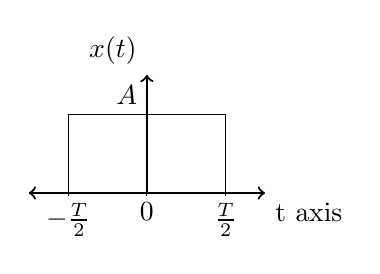
\begin{tikzpicture}
			\centering
			\draw[thick,<->] (-1.5,0) -- (1.5,0) node[anchor=north west] {t axis};
			\draw[thick,->] (0,0) -- (0,1.5) node[anchor=south east] {$x(t)$};
			\foreach \x in {-1,0,1}
			\draw (\x cm,1pt) -- (\x cm,-1pt) ;
			\foreach \y in {1}
			\draw (0,\y cm) -- (0,\y cm) node[anchor=south east] {$A$};
			\draw[black] (-1,0)node[anchor=north] {$-\frac{T}{2}$}--(-1,1) -- (1,1) -- (1,0)node[anchor=north] {$\frac{T}{2}$} ;
			\draw[black] (0,0)node[anchor=north]{$0$};
		\end{tikzpicture}
	\end{figure}
	This signal can be mathematically defined as:
	\begin{equation*}
		x(t) = A\left[ u(t+\frac{T}{2}) -u(t-\frac{T}{2})\right]
	\end{equation*}
	The Fourier transform of this signal would then be:
	\begin{equation*}
		X(\omega) = \int_{-\infty}^{\infty}\left[ A\left[ u(t+\frac{T}{2}) -u(t-\frac{T}{2})\right] e^{-i\omega t}dt
	\end{equation*}
	Because $x(t)$ is always equal to zero outside of the interval $\left[ -\frac{T}{2},\frac{T}{2}\right] $, we are allowed to change the limits of the integral.
	\begin{equation*}
		X(\omega) = \int_{-\frac{T}{2}}^{\frac{T}{2}}A e^{-i\omega t}dt
	\end{equation*}
	It is now trivial to evaluate the integral:
	\begin{align}
		X(\omega)&=\frac{A}{-i\omega}e^{-i\omega t} \bigg\vert_{-\frac{T}{2}}^{\frac{T}{2}}\\
		\label{eq:block:before}
		&= \frac{A}{-i\omega}(e^{-i\omega T/2}-e^{i\omega T/2})\\
		\label{eq:block:after}
        	&= {A}\frac{(-e^{-i\omega T/2}+e^{i\omega T/2})}{iw}\\
        	&= {AT}\frac{(-e^{-i\omega T/2}+e^{i\omega T/2})}{2iw\frac{1}{2}T}\\
		&= {AT}\frac{sin(\frac{\omega T}{2})}{{\frac{\omega T}{2}}}\\
		&=ATsinc(\frac{\omega T}{2})
	\end{align}
	Between step \ref{eq:block:before} and \ref{eq:block:after}, we made use of the following property:
	\begin{equation*}
		\sin(\frac{\omega T}{2}) = \frac{e^{i\omega T/2}-e^{-i\omega T/2}}{2i}
	\end{equation*}
\end{document}
